\chapter{Data Analysis}
\label{ch:dataanalysis}

\author{Nico Kratky}
%
\section {Regression Analysis}

Regression analysis is a statistical method to determine relationships between a response variable $ y $ and one or more predictor variables $ x_i $, where $ i = 1, 2, ..., p $. Linear regression analysis assumes that these predictor variables are related linear to the response variable.

\subsection{Simple Linear Regression}
\label{sec:slr}

Simple Linear Regression is a regression model that can only build a relationship between one predictor variable and one response variable. To find the best fit for this linear model the \textit{Ordinary Least Squares} method is used. The linear regression model builds a linear function

\begin{equation}
\label{eq:line}
    y = k * x + d
\end{equation}

that represents the predicted values. This function can also be denoted as

\begin{equation}
\label{eq:slr}
    y = \beta_0 + \beta_1 * x,
\end{equation}

where $ \beta_0 $ is the intercept and $ \beta_1 $ is the slope of the line.

The two regression parameters,

\begin{equation}
    \beta_1 = \frac{\sum_{i=1}^{n} (x_i - \bar{x}) * (y_i - \bar{y}))}{\sum_{i=1}^{n} (x_i - \bar{x})^2}
\end{equation}

\begin{equation}
    \beta_0 = \bar{y} - \beta_1 * \bar{x},
\end{equation}

that are used in this regression model are calculated using the least squares method. This method tries to minimize the sum of squared residuals.

\subsubsection{Example}

A good example for linear regression analysis is the ringsize of women. This example was taken from the website \url{http://www.crashkurs-statistik.de} \autocite{CrashkursSLR} \autocite{CrashkursMLR}.

If somebody wants to know the ringsize of his girlfriend, but does not want to ask her, it is possible to predict the size. To be able to do this a data basis has to be formed. A decisive factor for someones ringsize is for example the body height.

The data, which is depicted in table \vref{tab:slr_ringsize} can be used to calculate the regression coefficients using the formulae discussed in section \vref{sec:slr}. These calculations result in the two regression coefficients

\begin{equation}
    \beta_1 = \frac{\sum_{i=1}^{n} (x_i - \bar{x}) * (y_i - \bar{y}))}{\sum_{i=1}^{n} (x_i - \bar{x})^2} = 0.2838
\end{equation}

\begin{equation}
    \beta_0 = \bar{y} - \beta_1 * \bar{x} = 2.8457,
\end{equation}

which are slope and intercept, respectively.

\begin{table}[h]
    \centering
    \begin{tabular}{|l|l|l|l|l|l|l|l|l|l|l|}
    \hline
    \textbf{Person $ i $}    & \textbf{1} & \textbf{2} & \textbf{3} & \textbf{4} & \textbf{5} & \textbf{6} & \textbf{7} & \textbf{8} & \textbf{9} & \textbf{10} \\ \hline
    \textbf{Ringsize $ y $}  & 47.1       & 46.8       & 49.3       & 53.2       & 47.7       & 49.0       & 50.6       & 47.1       & 51.7       & 47.8        \\ \hline
    \textbf{Height $ x $}    & 156.3      & 158.9      & 160.8      & 179.6      & 156.6      & 165.1      & 165.9      & 156.7      & 167.8      & 160.8       \\ \hline
    \end{tabular}
    \caption{Ringsizes of example persons and their body heights}
    \label{tab:slr_ringsize}
\end{table}

After these calculations, the regression line can be plotted as shown in figure \vref{fig:slr_ringsize}.

\begin{figure}[h]
\centering
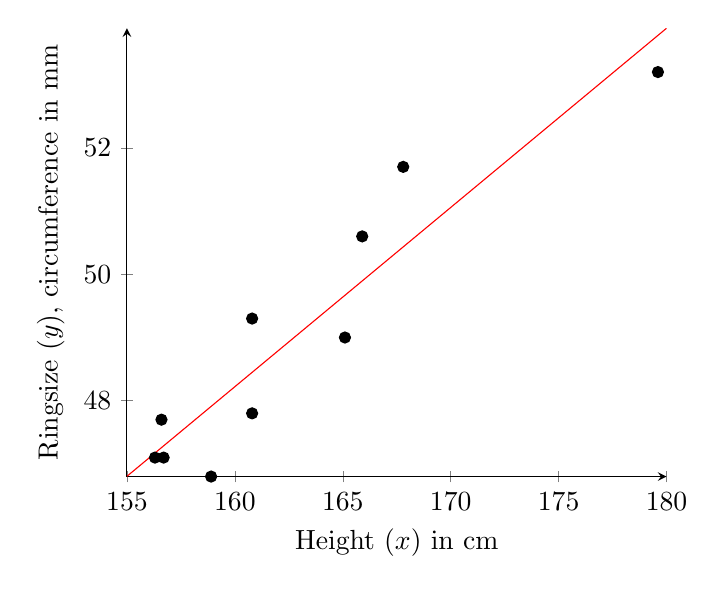
\begin{tikzpicture}
\begin{axis}[
    axis lines = left,
    xlabel = {Height ($x$) in cm},
    ylabel = {Ringsize ($y$), circumference in mm},
]
\addplot [
    domain=155:180,
    color=red
]
{2.8457 + 0.2836 * x};

\addplot[
    only marks
]
table {
    x       y
    156.3   47.1
    158.9   46.8
    160.8   49.3
    179.6   53.2
    156.6   47.7
    165.1   49.0
    165.9   50.6
    156.7   47.1
    167.8   51.7
    160.8   47.8
};

\end{axis}
\end{tikzpicture}

\caption{Ringsizes of women. The single data points represents the gathered data. The red line depicts the regression line.}
\label{fig:slr_ringsize}
\end{figure}

To predict a persons ringsize, two options are available. The first option, which is not as accurate as the second one, is to simple read the predicted value from the regression line. If, for example, a person is 165cm tall, the proper ringsize would be a little bit less than 50. To be more precise, the second option can be used, which is to calculate the size using the regression coefficients. This can be done by applying the regression line to the height

\begin{equation}
    y = 2.8457 + 0.2836 * 165,
\end{equation}

which yields $ y = 49.64 $.

\subsection{Multiple Linear Regression}
\label{sec:mlr}

When the dependent variable depends on not just one variable, multiple linear regression analysis is used. This method uses two or more independent variables to describe the dependent variable. To calculate the regression coefficients the predictor variables have to be put into a $ n \times p $ matrix,

\begin{equation}
    X_{n,p} =
        \begin{bmatrix}
            1 & x_{1,1} & x_{1,2} & \cdots & x_{1,p} \\
            1 & x_{2,1} & x_{2,2} & \cdots & x_{2,p} \\
            1 & \vdots & \vdots & \ddots & \vdots \\
            1 & x_{n,1} & x_{n,2} & \cdots & x_{n,p}
        \end{bmatrix}
\end{equation}

where $ n $ is the amount of datasets and $ p $ is the amount of predictor variables $ + 1 $ because the intercept also has to be calculated. Also, a vector of all response variables

\begin{equation}
    y_{n} =
        \begin{bmatrix}
            y_{1} \\
            y_{2} \\
            \vdots \\
            y_{n}
        \end{bmatrix}
\end{equation}

has to be formed. These two matrices can be used to describe the basic multiple linear regression model

\begin{equation}
    \begin{bmatrix}
        y_{1} \\
        y_{2} \\
        \vdots \\
        y_{p}
    \end{bmatrix}
    =
    \begin{bmatrix}
            1 & x_{1,1} & x_{1,2} & \cdots & x_{1,p} \\
            1 & x_{2,1} & x_{2,2} & \cdots & x_{2,p} \\
            1 & \vdots & \vdots & \ddots & \vdots \\
            1 & x_{n,1} & x_{n,2} & \cdots & x_{n,p}
    \end{bmatrix}
    \begin{bmatrix}
        \beta_{0} \\
        \beta_{1} \\
        \vdots \\
        \beta_{p}
    \end{bmatrix},
\end{equation}

where $ \beta $ are the regression coeffecients. Or shorter

\begin{equation}
    y = X\beta.
\end{equation}

\todo{describe what leads to the formula below (pseudoinverse, cite german uni paper)}

The problem with this equation is that it is possible that this equation does not have a solution. Therefore the $ y $ and $ X $ matrices are multiplied with the transpose of $ X $.

\begin{equation}
\label{eq:mlr}
    \hat{\beta} = (X^TX)^{-1} X^Ty
\end{equation}

\subsubsection{Example}

With this in mind, the example from section \vref{sec:slr} can be extended by more body parameters like weight and age, as they may also have an impact on the accuracy of the regression model. Figure \vref{tab:mlr_ringsize} depicts the ringsizes and body heights from the previous example, plus the weight and age of these people.

\begin{table}[H]
    \centering
    \begin{tabular}{|l|l|l|l|l|l|l|l|l|l|l|}
    \hline
    \textbf{Person $ i $}    & \textbf{1} & \textbf{2} & \textbf{3} & \textbf{4} & \textbf{5} & \textbf{6} & \textbf{7} & \textbf{8} & \textbf{9} & \textbf{10} \\ \hline
    \textbf{Ringsize $ y $}  & 47.1       & 46.8       & 49.3       & 53.2       & 47.7       & 49.0       & 50.6       & 47.1       & 51.7       & 47.8        \\ \hline
    \textbf{Height $ x_1 $}  & 156.3      & 158.9      & 160.8      & 179.6      & 156.6      & 165.1      & 165.9      & 156.7      & 167.8      & 160.8       \\ \hline
    \textbf{Weight $ x_2 $}  & 62         & 52         & 83         & 69         & 74         & 52         & 77         & 65         & 79         & 51          \\ \hline
    \textbf{Age $ x_3 $}     & 24         & 34         & 26         & 51         & 43         & 33         & 22         & 21         & 19         & 34          \\ \hline
    \end{tabular}
    \caption{Ringsizes of example persons and the appropriate body parameters}
    \label{tab:mlr_ringsize}
\end{table}

This dataset can now be used to form the previously explained matrices.

\begin{equation}
    X_{10, 3} =
    \begin{bmatrix}
        1 & 156.3 & 62 & 24 \\
        1 & 158.9 & 52 & 34 \\
        \vdots & \vdots & \vdots & \vdots \\
        1 & 160.8 & 51 & 34
    \end{bmatrix}
\end{equation}

\begin{equation}
    y_{10} =
    \begin{bmatrix}
        47.1 \\
        46.8 \\
        \vdots \\
        47.8
    \end{bmatrix}
\end{equation}

Using the regression parameter formula (see equation \vref{eq:mlr}) we get the regression parameters

\begin{equation}
    \hat{\beta} = (X^TX)^{-1} X^Ty =
    \begin{bmatrix}
        0.66 \\
        0.28 \\
        0.06 \\
        -0.02
    \end{bmatrix}.
\end{equation}

Using these parameters it is now possible to form the regression function

\begin{equation}
    y = 0.66 + 0.28 * x_1 + 0.06 * x_2 - 0.02 * x_3,
\end{equation}

which allows for data prediction.

In multiple linear regression analysis the predicted value can no longer be read off a graph, as the line is multi-dimensional. Lets assume that a woman is 170cm tall, weighs 68kg and is 29 years old. Inserting these values into the calculated model

\begin{equation}
    y = 0.66 + 0.28 * 170 + 0.06 * 68 - 0.02 * 29
\end{equation}

gives us the predicted ringsize $ y = 51.76 $.

\subsection{Working with Streaming Data}

As GRAMOC uses streaming data a few adjustements had to be made. The ordinary multiple linear regression model assumes that all observations are available when calculating the regression coefficients. Therefore a way of calculating these regression coefficients in a streaming way had to be found. To accomplish this the regression parameters have to be calculated incrementally. This means that the two parts of the regression parameter calculation, $ X^T X $ and $ X^T y $ have to be recalculated every time a new observation is made. These two matrices are then added up, since matrix addition between two $ n \times n$ matrices also result in a $ n \times n$ matrix. The sum of these matrices are named $ M $ and $ V $. This is possible as $ X^T X $ always returns a $ p \times p $ matrix and $ X^T y $ always returns a $ p $-dimensional vector.

When the regression coefficients are calculated,

\begin{equation}
    \hat{\beta_k} = (M + {X_k}^T X_k)^{-1}(V + {X_k}^T y_k),
\end{equation}

the sum of previous observation data is added to the current data, and then the procedure described in \vref{sec:mlr} can be applied.

This procedure was introduced in a regression calculation programm called StreamFitter, which also works with streaming data \autocite{StreamFitter}.

\subsection{$ r^2 $ - Coefficient of Determination}
\label{sec:rsquared}

$ r^2 $ is the quotient of the explained variation

\begin{equation}
    ESS = \sum_{i=1}^{n} (\hat{y}_i - \bar{y})^2
\end{equation}

and the total variation

\begin{equation}
    TSS = \sum_{i=1}^{n} (y_i - \bar{y})^2,
\end{equation}

\begin{equation}
    r^2 = \frac{ESS}{TSS}
\end{equation}

It is a measure for how much variation of the data can be explained with this regression model. $ r^2 $ values are ranged between $ 0 $ and $ 1 $, where $ 1 $ is considered a perfect fit and $ 0 $ says that no data can be explained using this regressino model.

\section{Implementation}

These procedures were implemented as a C++ class. The two most important methods from this class are \lstinline{void push(std::vector<double> X, double y)} and \lstinline{double predict(std::vector<double> X)}. The first method adds new observations to the model, and the second one tries to predict the response variable from the given predictor variables using the current linear regression model.

Code listing \vref{code:mlr_push} shows the \lstinline{push} method. Additionally to computing the $ M $ and $ V $ values, this method adds the variables to a queue-like data structure. This is necessary as the coefficient of determination needs the average of the response variable $ \bar{y} $ and the last few datasets to test this fit (see \vref{sec:rsquared}). The size of this structure is set to 100. This means that if the structure contains 100 datasets, the oldest one is removed before a new one is inserted.

\begin{minipage}{\textwidth}
\begin{lstlisting}[caption={C++ method to add new observations to the regression model},captionpos=b,label={code:mlr_push}]
void MLR::push(std::vector<double> X, double y) {
    if (X.size() != p_) {
        // not the correct amount of predictor variables
        return;
    }

    // add the values to a moving average and sliding window
    // this is used for calculating the coefficient of determination
    avg_y.add(y);
    sw_.add(std::make_pair(y, X));

    // create a 1x(p+1) matrix
    Eigen::Matrix<double, 1, Eigen::Dynamic> X2{p_ + 1};

    // insert values into matrix
    X.insert(X.begin(), 1);
    for (std::size_t i{0}; i < X.size(); ++i) {
        X2(0, i) = X[i];
    }

    auto X2T = X2.transpose();

    M_ = M_ + X2T * X2;
    V_ = V_ + X2T * y;

    // inserting new observations invalidates the coefficients
    coefficients_.clear();
}
\end{lstlisting}
\end{minipage}

Code listing \vref{code:mlr_predict} show the \lstinline{predict} method. This method initializes the result variable with the line intercept and then adds up the products of the predictor variable and the corresponding regression coefficient.

\begin{minipage}{\textwidth}
\begin{lstlisting}[caption={C++ method to predict the response variable using the passed predictor variables},captionpos=b,label={code:mlr_predict}]
double MLR::predict(std::vector<double> X) {
    if (X.size() != p_) {
        // not the correct amount of predictor variables
        return 0;
    }

    if (coefficients_.empty()) {
        // calculate coefficients if necessary
        calculate_coefficients();
    }

    // start prediction with the intercept
    double prediction = coefficients_[0];

    // add each predictor variable with its coefficient
    for (std::size_t i{0}; i < p_; ++i) {
        prediction += coefficients_[i + 1] * X[i];
    }

    return prediction;
}
\end{lstlisting}
\end{minipage}

\subsection{Matrix Calculations}

As the mathematical side of regression analysis requires a lot of calculations to be made using matrices and C++ does not have an equivalent to matrices, a third party library had to be chosen to compensate this. After comparing several linear algebra libraries that offer matrix calculations, it was decided to use Eigen.

\subsection{Eigen}

Eigen is a header-only C++ library, that was designed for doing basic linear algebra. This include matrix operations, vector calculations and numerical solvers. Its benefits include a very clean API which is fairly easy to use and a low memory overhead.

Perfomance-wise, Eigen is also better than its competitors.

\subsubsection{Benchmarks}

Figures \vref{fig:eigen_benchmark_ataT} and \vref{fig:eigen_benchmark_atv} depict the computational performance of Eigen. These two tests were done by computing the products of a matrix and its transpose and a matrix and a vector. When multiplying a matrix with its transponse, the GOTO BLAS library has a slight advantage over all matrix sizes but when multiplying matrices with vectors even the older version of eigen outperforms all competitors.

\begin{figure}[h]
    \centering
    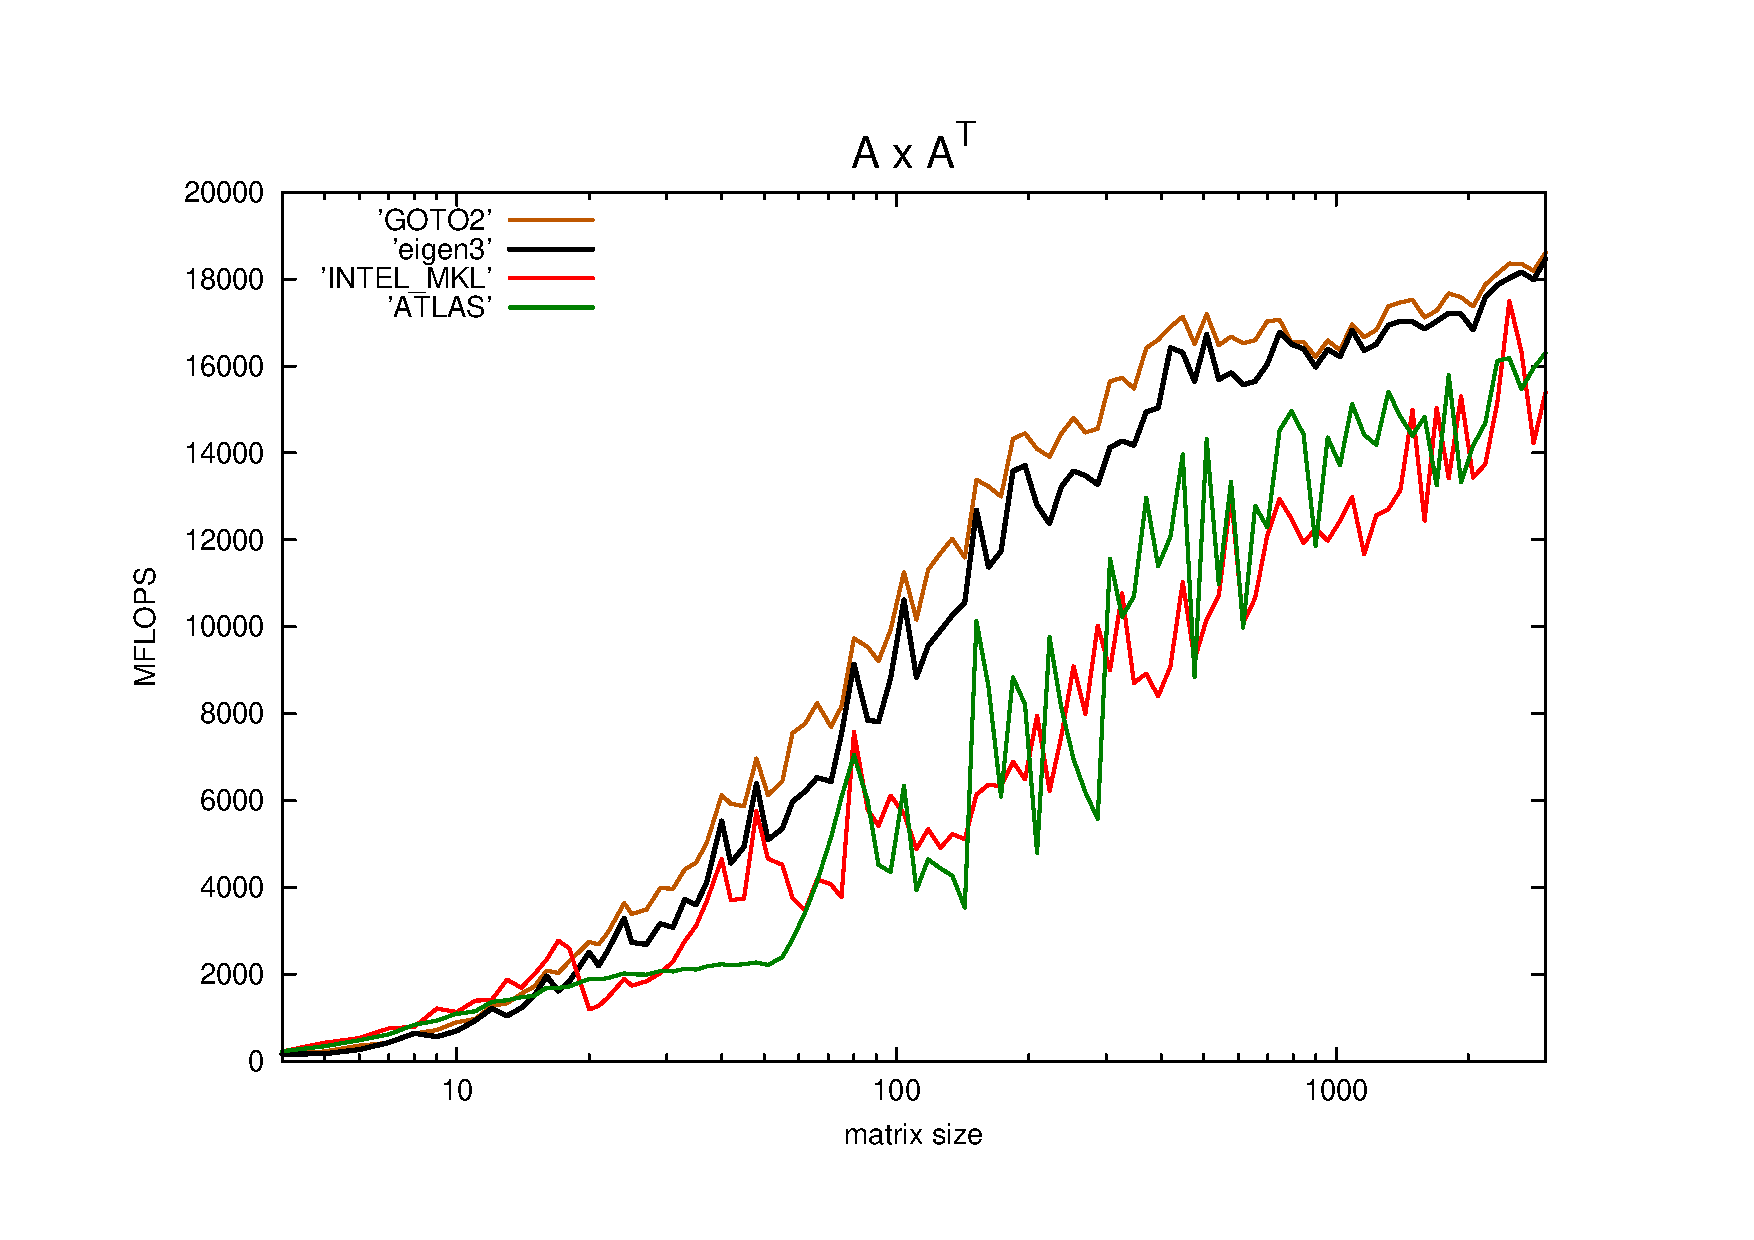
\includegraphics[width=0.8\textwidth]{eigen_benchmark_ataT}
    \caption{$ A \times A^T $ \autocite{EigenBenchmark}}
    \label{fig:eigen_benchmark_ataT}
\end{figure}

\begin{figure}[h]
    \centering
    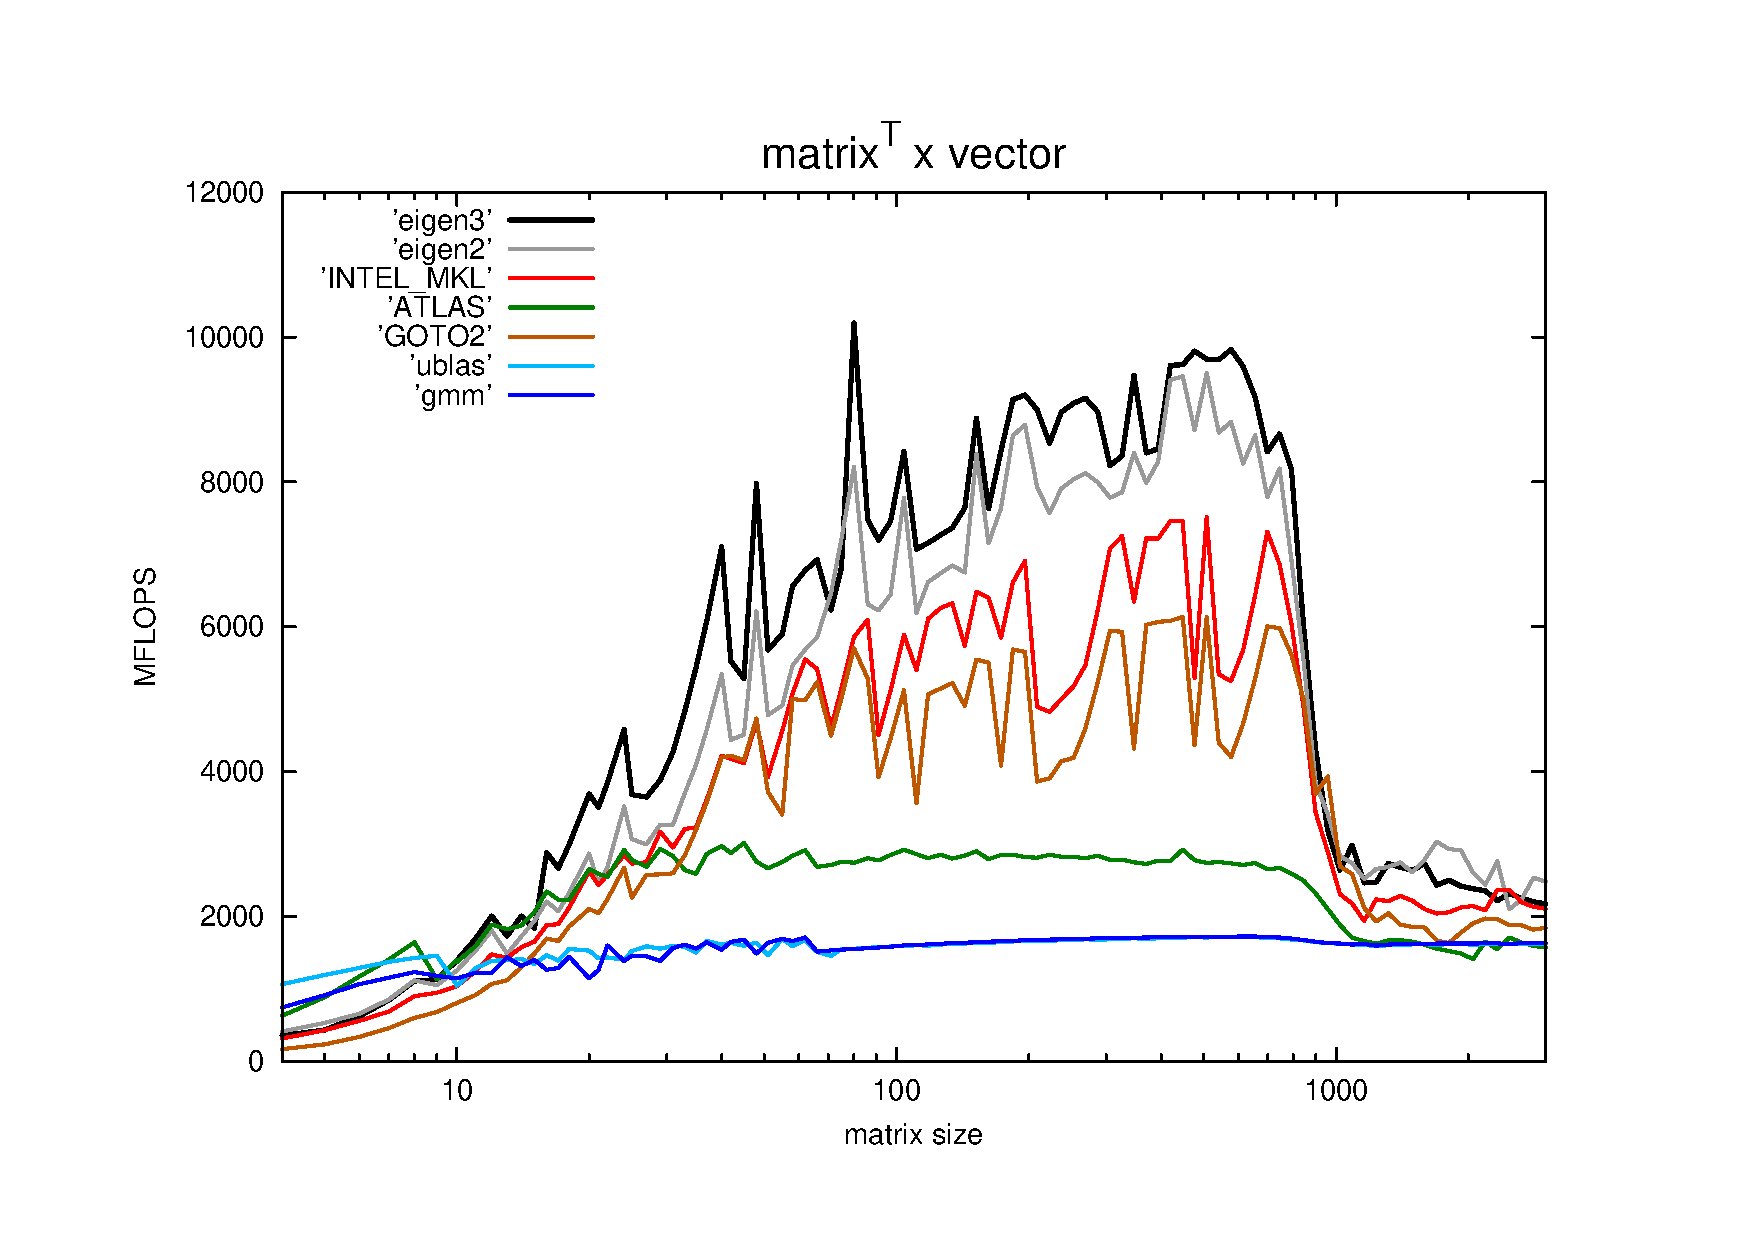
\includegraphics[width=0.8\textwidth]{eigen_benchmark_atv}
    \caption{$ matrix^T \times vector $ \autocite{EigenBenchmark}}
    \label{fig:eigen_benchmark_atv}
\end{figure}

